\documentclass[dvips,a4paper,12pt]{report}
\usepackage{xcolor}
\usepackage{float}
\usepackage{enumitem}
\usepackage{graphicx}
    \graphicspath{ {./img/} }
\usepackage[
    top=0.6in,
    bottom=0.6in,
    right=0.6in,
    left=0.6in]{geometry}

\begin{document}
\pagenumbering{arabic}


% ----------------------------------------- Begin content --------------------------------------------- %
%%% letter
\noindent Respected Examiner,

\noindent Thank you for reviewing my thesis.

\begin{center}
    \textbf{Thesis Title: Implementation of an Autonomous Star Recognition Algorithm using Hardware-Software Co-processing Approach} 
\end{center}

\noindent Firstly, I would like to thank you for your insightful comments. These excellent comments have helped significantly improve my thesis. This letter addresses each of the raised points and notes precisely how I have responded and included the comments into my revised thesis. \\

\vspace{0.5in}

\noindent Sincerely yours,

\noindent Dang Le Dang Khoa

%%% Q&A
\newpage

\color{blue}
\noindent \large{\textbf{Examiner: 2}}

\begin{enumerate}
    \color{blue}
    \item There are many careless mistakes in the thesis. Tables and figures are not explained in the body of the thesis, equations are given without explanations, unfinished sentences, etc. All these are indicated on the relevant pages in the thesis. Please correct and give explanations as requested.

    \color{black}
    Thanks for pointing these out in your ``Additional Document'' file. I have checked and fixed them all. I also have amended detailed explanations and restructured Chapter 3 and 4. \\

    \color{blue}
    \item Page 29. Please explain why the threshold is chosen to be 70 to separate star clusters from the background. What will happen if the threshold is reduced or increase?

    \color{black}
    I have amended a precise explanation to chapter 3.3.1 Centroiding (pages: 28,29,30). To summarize how to choose the threshold value:

    \begin{itemize}
        \item Firstly, I perform an analysis by averaging and counting the occurences of all pixel values in the star image dataset. 
        \item The result of the analysis would form a pattern which is shown like the below image. It includes 2 significant clusters: the first cluster is the background pixel values which formed near 0 Intensity value and the second cluster is the star pixel value which formed near the 255 Intensity value and scattered data points in between(which represent the noise)
        \item Based on the analysis, We know the range of threshold value is in between the noise values and the star pixel cluster.
        \item Finally, while carrying out experiments on the test dataset, we fine-tune and optimize the threshold value to produce the highest possible accuracy.
    \end{itemize}

    \begin{figure}[H]
        \centering
        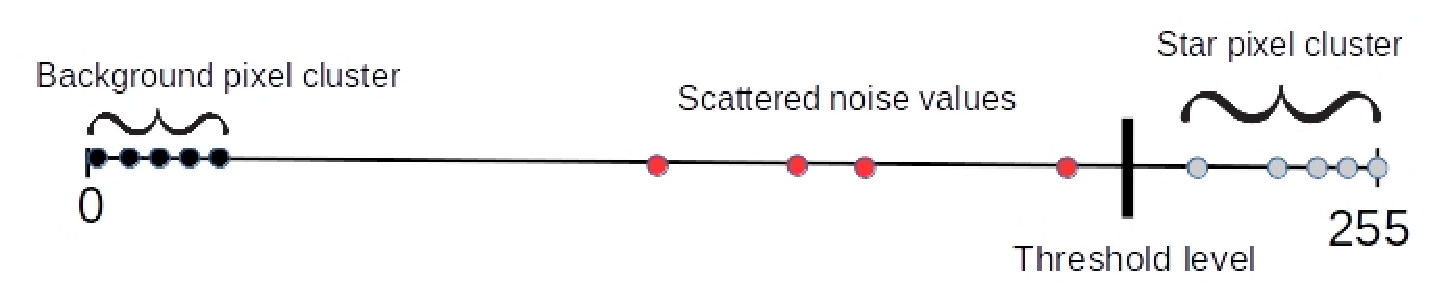
\includegraphics[width=1.0\textwidth]{4}
    \end{figure}

    If we set the threshold too low, it would lead to mismatches. Otherwise, if we set the threshold too high, some stars would be missing from the image.

    \color{blue}
    \item Conclusion must be made for the study, so I would like to see a chapter on conclusion which includes the following:

    \begin{enumerate}[label=(\alph*)]
        \color{blue}
        \item One of the objective of the candidate's thesis is to implement and evaluate the performance of a star tracking algorithm, so what is the conclusion of the evaluation of the performance? Can it be used for the attitude determination sensor mounted on a spacecraft?

        \color{black}
        I have amended some details to the summary and future works in Chapter 5. For the question ``Can it be used for the attitude determination sensor mounted on a spacecraft?'', based on the final Runtime Comparison results, the answer is yes since the runtime meet the requirements. In the future works section, I suggested a depth study on noise to implement a hardware module that performs the noise cancellation efficiently since my implementation only deals with basic noise. Furthermore, we need an autonomous input-processing module that can manage a large stream amount of images to meet the processing rate and improve the throughput. (This task would be depended on each specific spacecraft). \\

        \color{blue}
        \item Another objective of the thesis is to benchmark and optimize the algorithm in terms of the power consumption and the area of transistor implementation. What is the conclusion? What is the benchmark now? Did the candidate do optimization? What I got from the thesis are just the results of the power consumed, but it is necessary that the candidate describes how he did the optimization.

        \color{black}
        I have amended some details to Chapter Hardware design(restructured to Chapter 4.2 from page 45 to page 48). I have added a conclusion that the hardware-software co-processing approach is advantageous than the software-only approach in term of power consumption. 

        The hardware design is written on a high-level language and relied on specific Xilinx design rules and optimizations like Loop pipelining to enhance the processing speed. My optimization was mostly done in the algorithmic level like transfer dependant loops to independent loops, transfer array index to a stream and indexing by the binary search to reduce BRAM storages. Since they are technical and specific, I would not prefer to include in the thesis. An optimization has been mentioned in the thesis is using the one-pass scan algorithm to solve the connected component problem without using complicated data structures to reduce the hardware runtime. \\

    \end{enumerate}

\end{enumerate}



% ----------------------------------------- End content --------------------------------------------- %
\end{document}
